Let's briefly recap the key definitions that have been covered so far in the lectures. The position of a particle is generally expressed as the vector ${\bf r}(t)$. Then the velocity is ${\bf v}(t)=\dot{\bf r}(t)$ and the acceleration is ${\bf a}(t)=\ddot{\bf r}(t)$.

\begin{itemize}
  \item The {\em angular speed} of a particle is denoted $\omega(t)=\dot{\theta}(t)$, and is the rate of change of $\theta$ at time $t$.  For general motion $\omega(t)=\frac{|{\bf v}_{\perp}(t)|}{{\bf r}(t)}=\frac{|{\bf r}(t)\times{\bf v}(t)|}{|{\bf r}(t)|^{2}}$.
		   \begin{center}
                   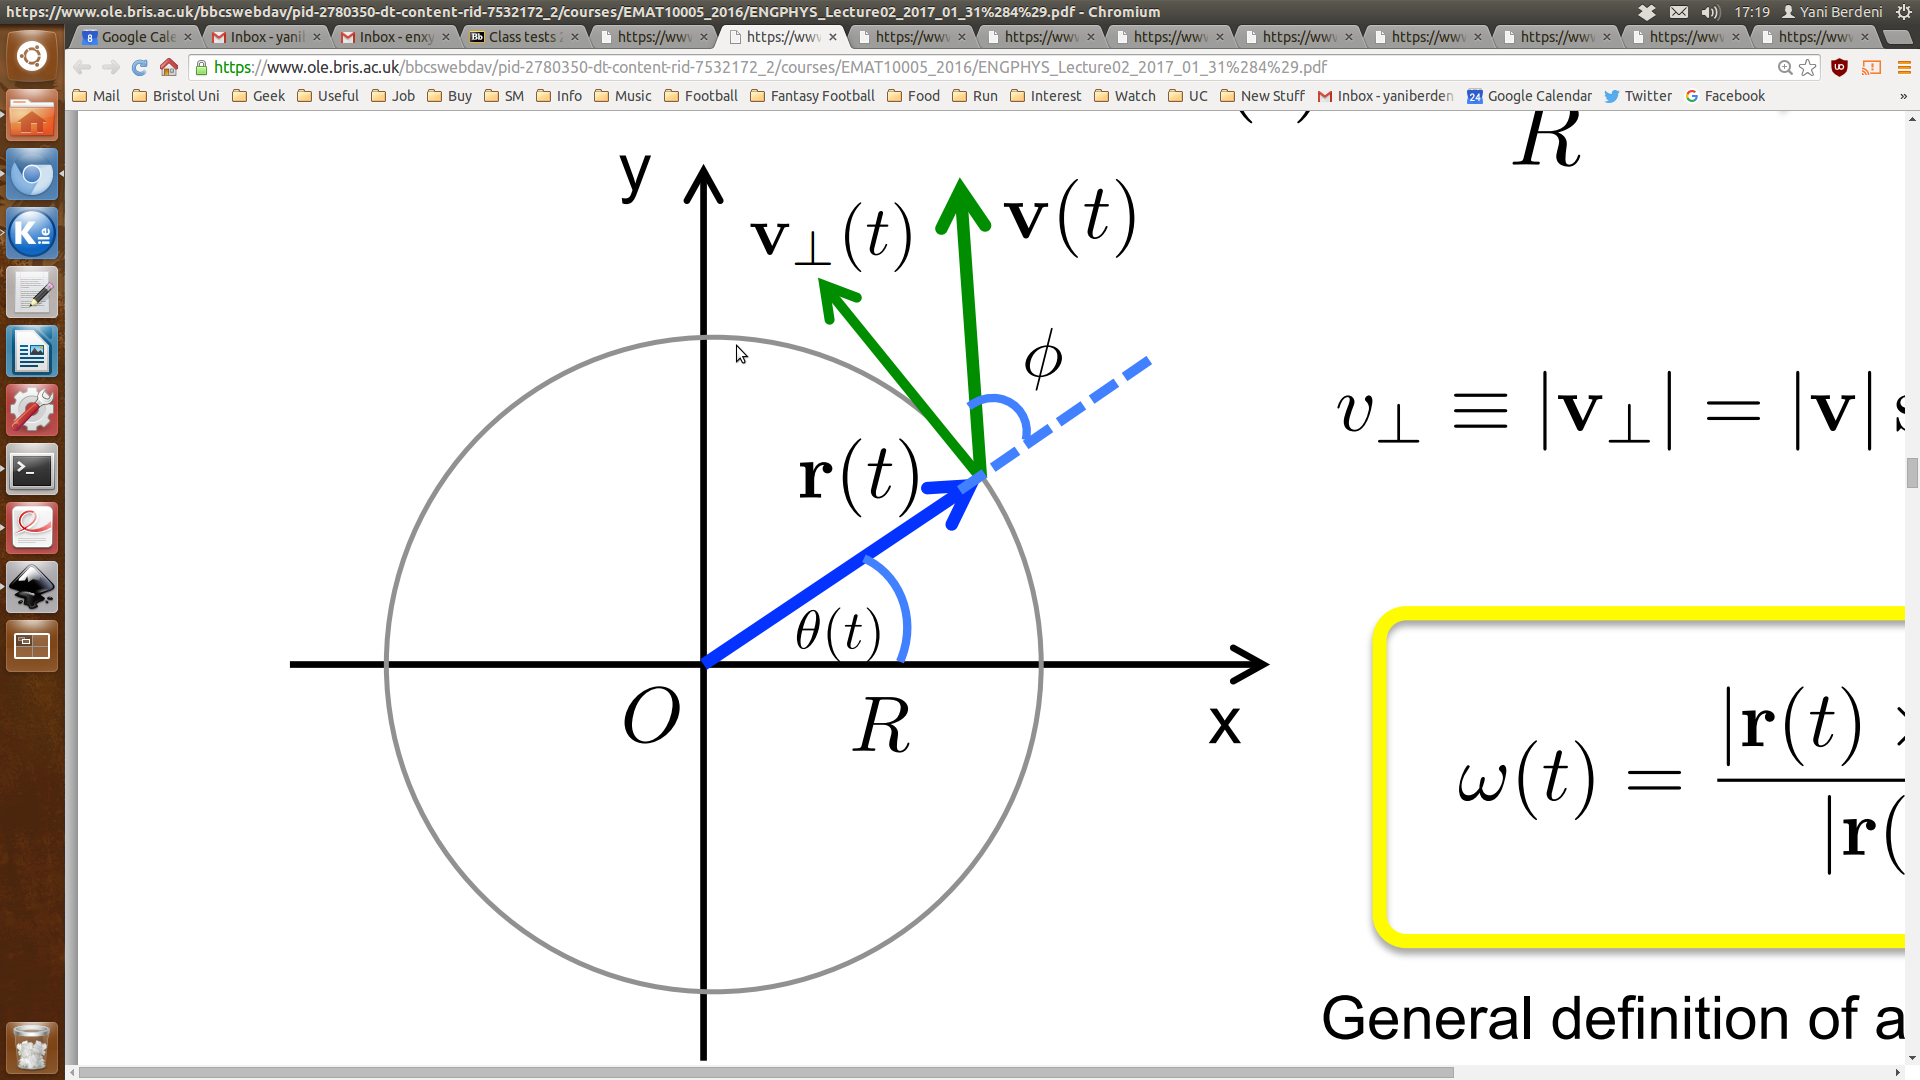
\includegraphics[width=0.28\textwidth]{preamble.pdf}
                   \end{center}

  \item The {\em angular velocity} of a particle $\boldsymbol{\omega}(t)$ is a vector of magnitude equal to the angular speed $\omega(t)$ and direction perpendicular to the plane of rotation.  It is given by $\boldsymbol{\omega}(t)=\frac{{\bf r}(t)\times{\bf v}(t)}{|{\bf r}(t)|^{2}}$.
          \begin{center}
        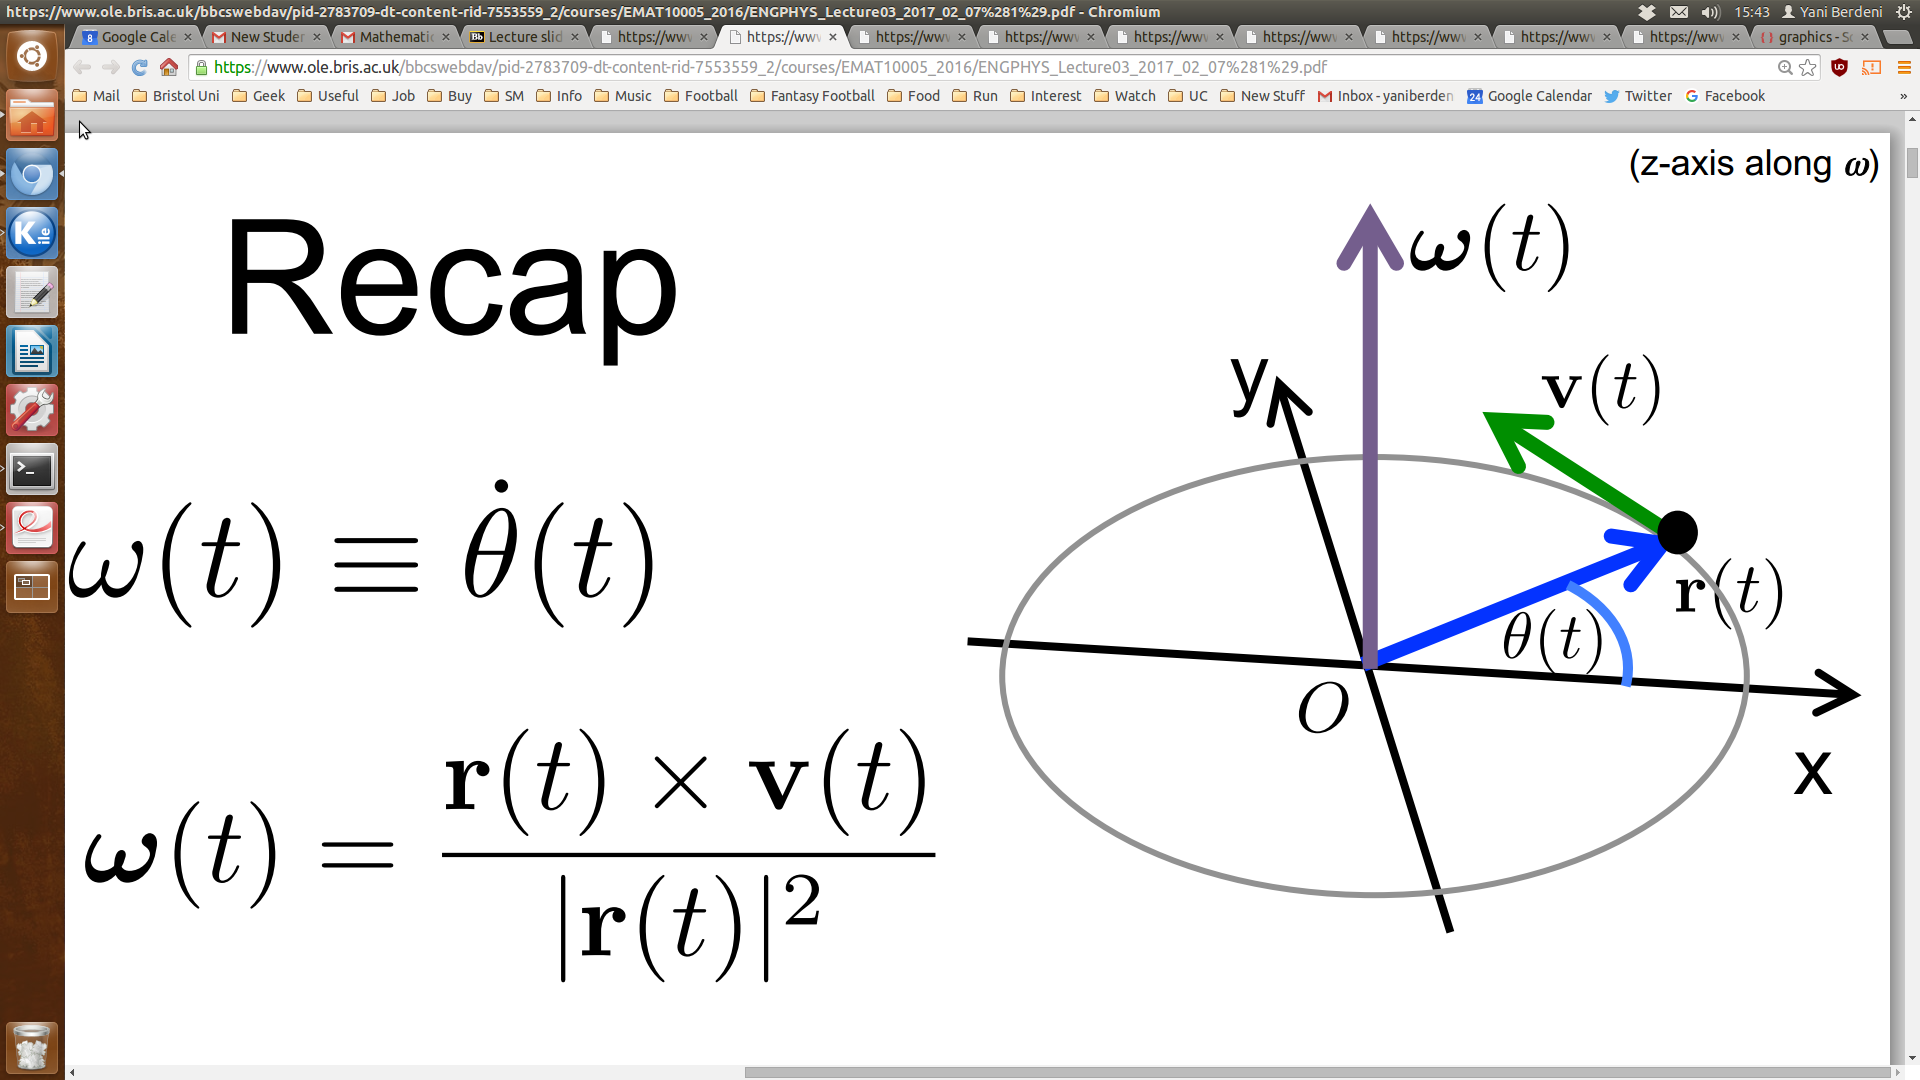
\includegraphics[width=0.25\textwidth]{preamble1.pdf}
        \end{center}
 
 \item For circular motion the angular velocity is given by ${\bf v}(t)=\boldsymbol{\omega}(t)\times {\bf r}(t)$. The angular speed is given by $|{\bf v}(t)|=v(t)=\omega(t) R$.
 
  \item The {\em linear momentum} of a point particle is the product between the mass and velocity of the particle, ${\bf p}(t)=m{\bf v}(t)$. From Newton's 2nd Law, it follows that the resultant force is the time derivative of the linear momentum: ${\bf F}(t)=\frac{d}{dt}{\bf p}(t)$.
  \item {\em Impulse} is the integral of the resultant force over a time interval: ${\bf J}(t_{0},t_{1})=\int_{t_{0}}^{t_{1}} {\bf F}(t) dt$. The Impulse-Momentum Theorem states that the impulse is equal to the change in momentum: \newline ${\bf J}(t_{0},t_{1})={\bf p}(t_{1})-{\bf p}(t_{0})$.
  \item The {\em angular momentum} of a particle relative to origin $O$ is given by ${\bf H}_{O}(t)={\bf r}(t)\times {\bf p}(t)=m |{\bf r}(t)|^{2}\boldsymbol{\omega}(t)$. It points in the same direction as the angular velocity.
  \item The {\em torque} of a force ${\bf F}(t)$ relative to origin $O$ is given by ${\bf M}_{O}(t)={\bf r}(t)\times {\bf F}(t)$. Provided $O$ is fixed (${\bf v}_{O}=0)$), the torque is the time derivative of the angular momentum: ${\bf M}_{O}(t)=\frac{d}{dt}{\bf H}_{O}(t)$.
  
  \item The {\em work} done by a force ${\bf F}$ along path $C$ between $P_{1}$ and $P_{2}$ is:  $W_{C}^{(F)}(P_{1},P_{2})=\int_{P_{1}}^{P_{2}}{\bf F} \cdot {d {\bf r}}$.
    
          \begin{center}
        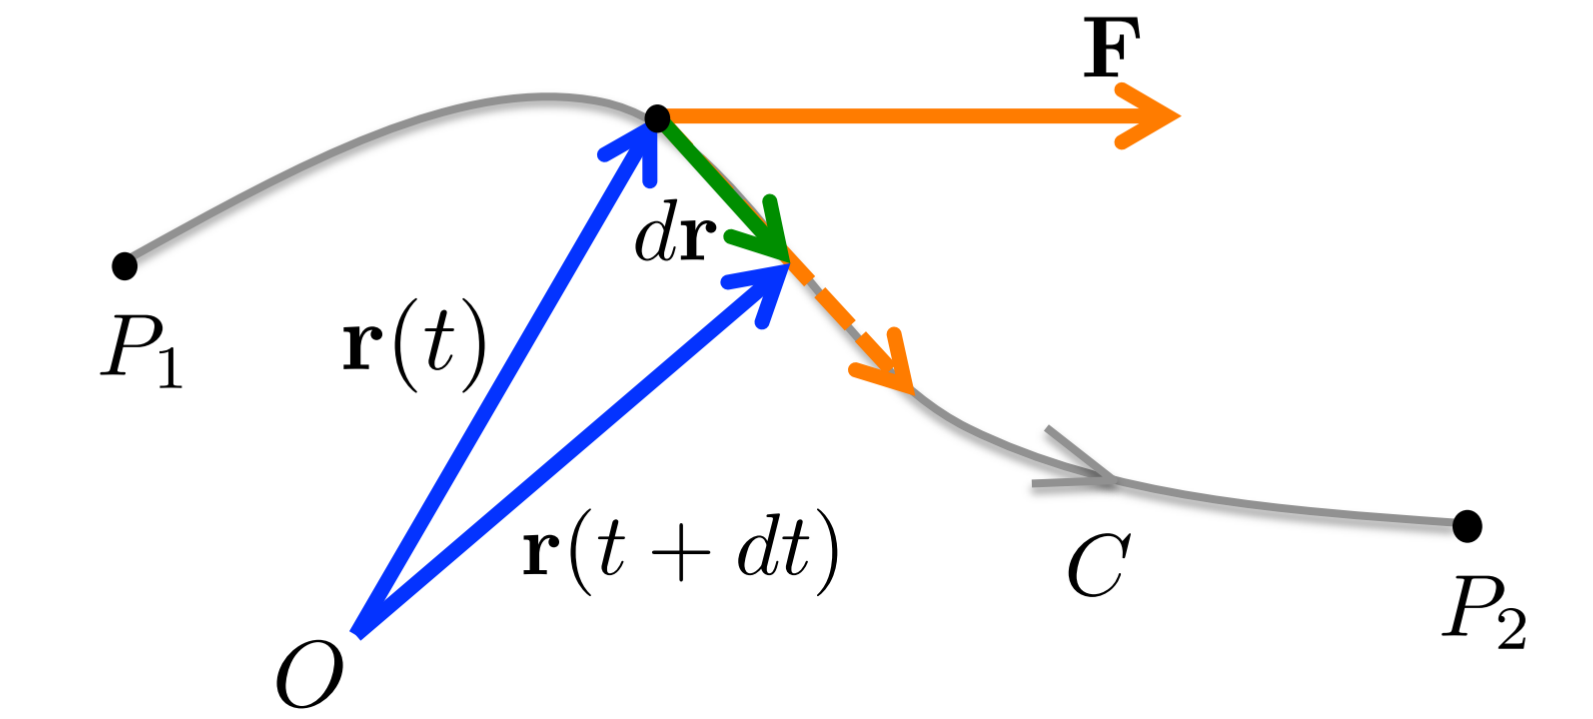
\includegraphics[width=0.37\textwidth]{preamble2.pdf}
        \end{center} 
  
  \item The Work-Energy Theorem states that the work of the resultant force is equal to the change of kinetic energy: $W_{C}^{(F)}(t_{1},t_{2})=T(t_{2})-T(t_{1})=\frac{1}{2}m \left ( v^{2}(t_{2})-v^{2}(t_{1}) \right )$.
\end{itemize}